\documentclass[conference,a4paper]{IEEEtran}
% pdflatex sladen-eol2017-tunnels && bibtex sladen-eol2017-tunnels && pdflatex sladen-eol2017-tunnels && evince sladen-eol2017-tunnels.pdf
% https://easychair.org/conferences/submission.cgi?submission=3128849;a=13821857
\usepackage[colorlinks=false,pdfborder={0 0 0}]{hyperref}
\hypersetup{
  colorlinks=false,
  pdfborder={0 0 0},
  pdfauthor={Paul Sladen},
  pdftitle={Tunnels of Knowledge: Mapping today's 'secrets' from Yesterday's public maps},
  pdfsubject={Exploring Old Maps (2017), W{\"u}rzburg},
  pdfkeywords={Channel Tunnel; Citizen science; Crowdsourcing; London Underground; OpenStreetMap; Public safety; Public transport; Tunnels; Underground infrastructure},
  pdfcreator={Paul Sladen},
  pdfproducer={Emacs, pdflatex, bibtex, JOSM, Gimp, pdfimage},
  pdflang=en,
  pdfcreationdate=D:20170201101000+00'00',
  pdfmoddate=D:20170331113000+02'00',
  pdfencoding=unicode
}
\usepackage[all]{hypcap}
\usepackage[pdftex]{graphicx}
%\usepackage[cmex10]{amsmath}
\usepackage[noadjust]{cite}
\usepackage{cite}
\usepackage{url}
\hyphenation{op-tical net-works semi-conduc-tor}
\usepackage{filecontents}

\begin{filecontents}{sladen-eol2017-tunnels2.bib}
@IEEEtranBSTCTL{IEEEtweaked:BSTcontrol,
  CTLdash_repeated_names = "no",
}

@article{sladen-sotm2013,
  author  = {{Paul} Sladen}, 
  title   = {{Tube to Chunnel---Underground Mapping}},
  journal = {State of the Map},
  year    = 2013,
  month   = Sep,
  url = {http://lanyrd.com/2013/sotm/scpkgy/},
  organization = {OpenStreetMap},
  type = {Talk},
}

@article{foi-2011,
  author = {Robin Taylor and {London Underground}},
  title = {{Location of Mid Tunnel Vent Shafts and Intervention Points}},
  journal = {WhatDoTheyKnow},
  year = 2011,
  month = Oct,
  note = {{Freedom of Information} request},
  url = {https://www.whatdotheyknow.com/request/location_of_mid_tunnel_vent_shaf},
}

@thesis{darroch-2012,
  author = {Nathand Darroch},
  organization = {University of York},
  year = 2012,
  month = Sep,
  title = {London's Deep Tube Railways: Visibly Invisible},
  url = {http://etheses.whiterose.ac.uk/3905/1/London%E2%80%99s_Deep_Tube_Railways-_Visibly_Invisible,_Nathan_Darroch.pdf},
  type = MA,
  note = {{MA by research}},
}

@article{darroch-2014,
  author = {Nathan Darroch},
  title = {{A brief introduction to London's underground railways and land use}},
  journal = {Journal of Transport and Land Use},
  volume = 7,
  number = 1,
  year = 2014,
  pages = {105--116},
  doi = {10.5198/jtlu.v7i1.411},
  url = {http://econpapers.repec.org/RePEc:ris:jtralu:0124},
}
%%  url = {https://www.jtlu.org/index.php/jtlu/article/download/411/402},

@misc{openstreetmap,
  author = {{OpenStreetMap contributors}},
  title = {OpenStreetMap geo database},
  howpublished = "\url{http://www.openstreetmap.org}",
  year = {2004--2017},
}

@report{riab-2013,
  author = {{Rail Accident Investigation Branch}},
  title = {{Penetration and obstruction of a tunnel between Old Street and Essex Road stations, London 8 March 2013}},
  url = {https://assets.publishing.service.gov.uk/media/547c8fb940f0b60241000157/R032014_140213_Old_Street.pdf},
  year = 2014,
  month = Mar,
  note = { ``Railway Infrastructure Managers with tunnels and associated
subterranean structures which are under urban areas ... should then take all reasonable
steps to publicise this information,''},
}

%  note = {``Railway Infrastructure Managers with tunnels and associated
% subterranean structures which are under urban areas and not shown
% on Ordnance Survey mapping should implement a process to publish
% information concerning those areas of land that are in reasonable
% proximity to this infrastructure. They should then take all reasonable
% steps to publicise this information,''},


@report{riab-2010,
  author = {{Bureau d'enquêtes sur les Accidents de transport terrestre} and {Rail Accident Investigation Branch}},
  title = {{Technical Investigation Report concerning the Fire on Eurotunnel Freight Shuttle 7412 on 11 September 2008}},
  url = {https://assets.publishing.service.gov.uk/media/547c900c40f0b60244000185/101122_ReportET2010_eurotunnel_eng.pdf},
  year = 2010,
  month = Nov,
  note = { ``Only knowing the PK at which mission 7412 has stopped, he
    looks for the corresponding cross-passage number in the tunnel
    pocket book. This takes about two minutes.''}
}

@report{riab-2016,
  author = {{Bureau d'enquêtes sur les Accidents de transport terrestre} and {Rail Accident Investigation Branch}},
  title = {{Technical Investigation Report: Concerning the fire on Eurotunnel freight shuttle 7340 on 17 January 2015}},
  url = {https://assets.publishing.service.gov.uk/media/572b0031ed915d1452000000/160505_ReportET2016_eurotunnel_eng.pdf},
}

@report{eurostar,
  title = {{Eurostar Independent Review}},
  year = 2010,
  month = Feb,
  url = {http://www.railwaysarchive.co.uk/documents/Garnett_EurostarIndependentReview2010.pdf},
  note = { ``As the train was located close to the crossover between
    the two running tunnels, passengers were required to enter through
    a cross passage door, and negotiate up a staircase to reach the
    service tunnel, proceed along the service tunnel to another cross
    passage door through which the recovery shuttle was be
    accessed. There was a distance of 375 metres between the
    platforms.''}
}

@misc{foi-2015,
  url = {https://www.whatdotheyknow.com/request/maps_of_public_corridors_on_larg},
  title = {{Maps of public corridors on larger Tube stations}},
  work = {{WhatDoTheyKnow}},
  author = {{Georg Vehres} and {{Transport for London}}},
  year = 2015,
  month = June,
}

@thesis{street-2006,
  author = {Nicholas Street},
  title = {{TimeContours: Using isochrone visualisation to describe transport network travel cost}},
  note = {Final Report},
  month = Jun,
  year = 2006,
  url = {http://www.imperial.ac.uk/pls/portallive/docs/1/18619712.PDF},
}

@misc{osm-wiki-chunnel,
  author = {Paul Sladen},
  title = {{Channel Tunnel}},
  journal = {{{OpenStreetMap}} wiki},
  url = {https://wiki.openstreetmap.org/wiki/Channel_Tunnel},
  note = {{Numerical constraints}},
  year = {2013--2017},
}

@article{korittke-1989,
  author = {Norbert Korittke},
  year = 1989,
  title = {{Influence of horizontal Refraction on the traverse Measurements in Tunnels with Small Diameters}},
  organization = {{Bochum, W-Germany: Institute for Deposits and Surveying, DMT}},
  pages = {13--17},
  url = {http://www.slac.stanford.edu/econf/C9009106/papers/023.PDF}
}

@thesis{korittke-1997,
  author = {Norbert Korittke},
  year = 1997,
  title = {{Zur Anwendung hochpr{\"a}ziser Kreiselmessungen im Bergbau und Tunnelbau}},
  page = 131,
  note = {Doctoral thesis, {ISBN:} 3-926146-09-5},
  organization = {Technische Universität Braunschweig},
  ISBN = {3-926146-09-5},
}
\end{filecontents}
\renewcommand{\citedash}{--} 
\begin{document}
\bstctlcite{IEEEtweaked:BSTcontrol}
\vspace{-1em}
\title{\hphantom{:}Tunnels of Knowledge:\\
\vspace{-0.6em}
{\Large \hphantom{'}Mapping today's `secrets'\\\vspace{-0.8em} from Yesterday's public maps}\\
\vspace{-0.2em}{\large *\,(and improving public safety)\hphantom{\,*}}}
\author{%
  \texorpdfstring{%
    \IEEEauthorblockN{Paul Sladen}
    \IEEEauthorblockA{Astronomical Calculation Institute (ARI--ZAH), University of Heidelberg\\\small\texttt{sladen@\{ari.uni-heidelberg.de,gmail.com\}}}
}{Paul Sladen}}
\maketitle

\begin{IEEEkeywords}
Channel Tunnel.
Citizen science.
Crowdsourcing.
London Underground.
OpenStreetMap.
Public safety.
Public transport.
Tunnels.
Underground infrastructure.
\end{IEEEkeywords}

\IEEEpeerreviewmaketitle

%\vspace{1.25em}
\section{Introduction}
Everyday millions of people travel by U-Bahn, Metros, subways and the
Tube. Most travel in a blinded fashion, steered through a brightly-lit
linear maze, and unaware of where they are. Modern society often
choses actively or passively to restrict maps of underground
infrastructure, even when it is open for all. This is in contrast to
the social dynamics of the early 1900s, when engineers were
enthusiastic to share and the public eager to absorb.

OpenStreetMap~\cite{openstreetmap} is a worldwide geo-database containing a contributed and
crowdsourced vector dataset along with textual metadata, quickly making it one
of the largest datasets available for research and analysis~\cite{street-2006}. For
citizens involved with mapping transport and underground metro
systems, use of old out-of-copyright maps allows obtaining and
rescuing information otherwise unavailable in the modern world. The
presentation will show mapping of features from the complex London
Underground system using old parliamentary maps as a basis; and
efforts for precision mapping of the Channel Tunnel using custom
software written to reproject numerical tables of engineering
survey data---where existing libre software 
for projecting absolute azimuth/distance measurements into WGS\,84 coordinates was not found readily available.

\vspace{0.4em}
%\vspace{1em}
\section{Tunnelling towards openness}
%\vspace{0.5em}
Following incidents in both London and the Channel~Tunnel, official
reports from the public humanities investigating the handling of the
incidents have highlighted lack of available information as a
significant contributing factor~\cite{riab-2010,riab-2013,openstreetmap,foi-2011}. Yet,
other players continue to advocate for non-publication in digital
media form~\cite{foi-2011}. Using historical maps via digitisation, a
[citizen] transport user can proactively enact official
recommendations to improve public safety by dissemination of
information. For myself, as an OpenStreetMap
practitioner with a background in programming and an active interest
in open knowledge, the possibility of citizen science being able to
have direct agency through the use of old maps is intriguing.\par\vspace*{\fill}

\subsection{London Underground}\vspace{-0.2em}

During the 2010s a member of London Underground's Infrastructure
Protection team began research for their own MA and PhD theses.  The
published papers resulting contain many examples contrasting historic
maps with output from London Underground's internal infrastructure
maps~\cite{darroch-2012,darroch-2014}. The allowance for
including internal London Underground maps is perhaps an indication of a
more open attitude by London Underground.  Having such plans enables the opportunity for
comparision against OpenStreetMap, but also the possibility of
tainting OpenStreetMap.  During one comparison a substantial difference was observed---when queried it was confirmed that the
alignment on OpenStreetMap was correct, and it was the 
London Underground's internal maps that were out-of-date.

In 2015 Transport for London released additional quasi-{\small 3D} (axonometric) diagrams of
the internal structure of most of the underground stations~\cite{foi-2015}.
This caused additional information to fall into the public {\it knowledge}
domain---but not necessarily into the public domain of (legally usable) information and
data available for freely-using.  OpenStreetMap must therefore still
turn to information that is truely out-of-copyright.\hfill{}\hyperref[fig:south-ken-bends]{[Fig.\,1]}\\
Luckily, many of the metro and underground railways were constructed in the
1900s--1920s meaning original construction plans have
fallen out of copyright and can be safely used as a research base for digital mapping.

%\vspace{-0.7em}%
\subsection{Channel Tunnel}%
\vspace{-0.112em}

This international undersea tunnel was designed in the 1980s,
privately constructed, and opened in the early-1990s.  Plans and maps
remain in copyright, split between Eurotunnel, and the various private
construction companies.  An entirely different approach has
been applied, tabulating individually published numerical
constraints (spacing, lengths, radii) to recreate a virtual survey~\cite{osm-wiki-chunnel,sladen-sotm2013}.
Publications cover
survey traverses performed using gyrotheodolite, first along the tunnel walls, then secondly along the centre-line---%
to avoid a newly-observed problem of horizontal
refraction caused by temperature gradients in the air at the tunnel walls~\cite{korittke-1997,korittke-1989}.
We confirm correct re-projection into WGS\,84 of the surveys by observing
one zig-zagging around the other traverse.~\hfill\hyperref[fig:osm-chunnel-traverse]{[Fig.\,2]}\par\vspace*{\fill}

\begin{figure*}[!lt]
  \centering
  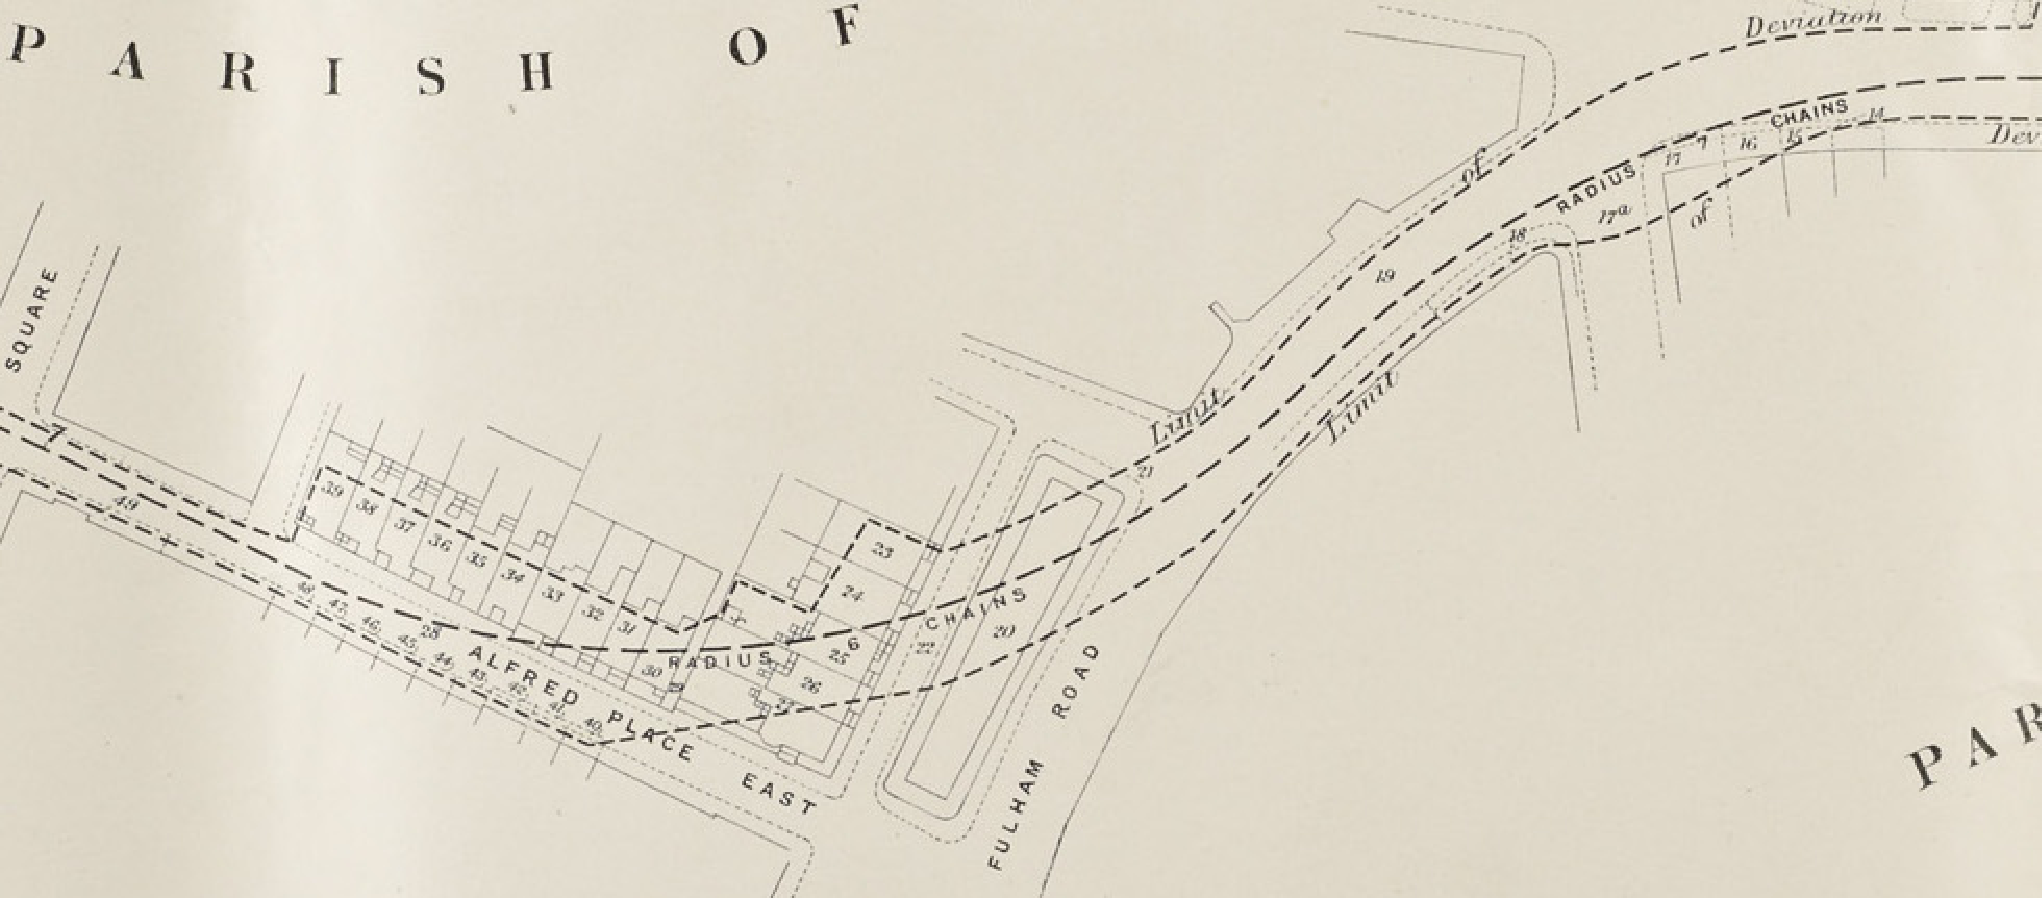
\includegraphics[width=15.1cm]{reverse-curves-cropped}
  \vspace{-0.5em}
  \caption{London Underground (1897 submitted plans) later the Piccadilly line.  Development of ``South Kensingtons Bends'' double S-curves under highway.\hfill}
  \label{fig:south-ken-bends}
\end{figure*}
\vspace{-1em}
\begin{figure*}[!lt]
  \centering
  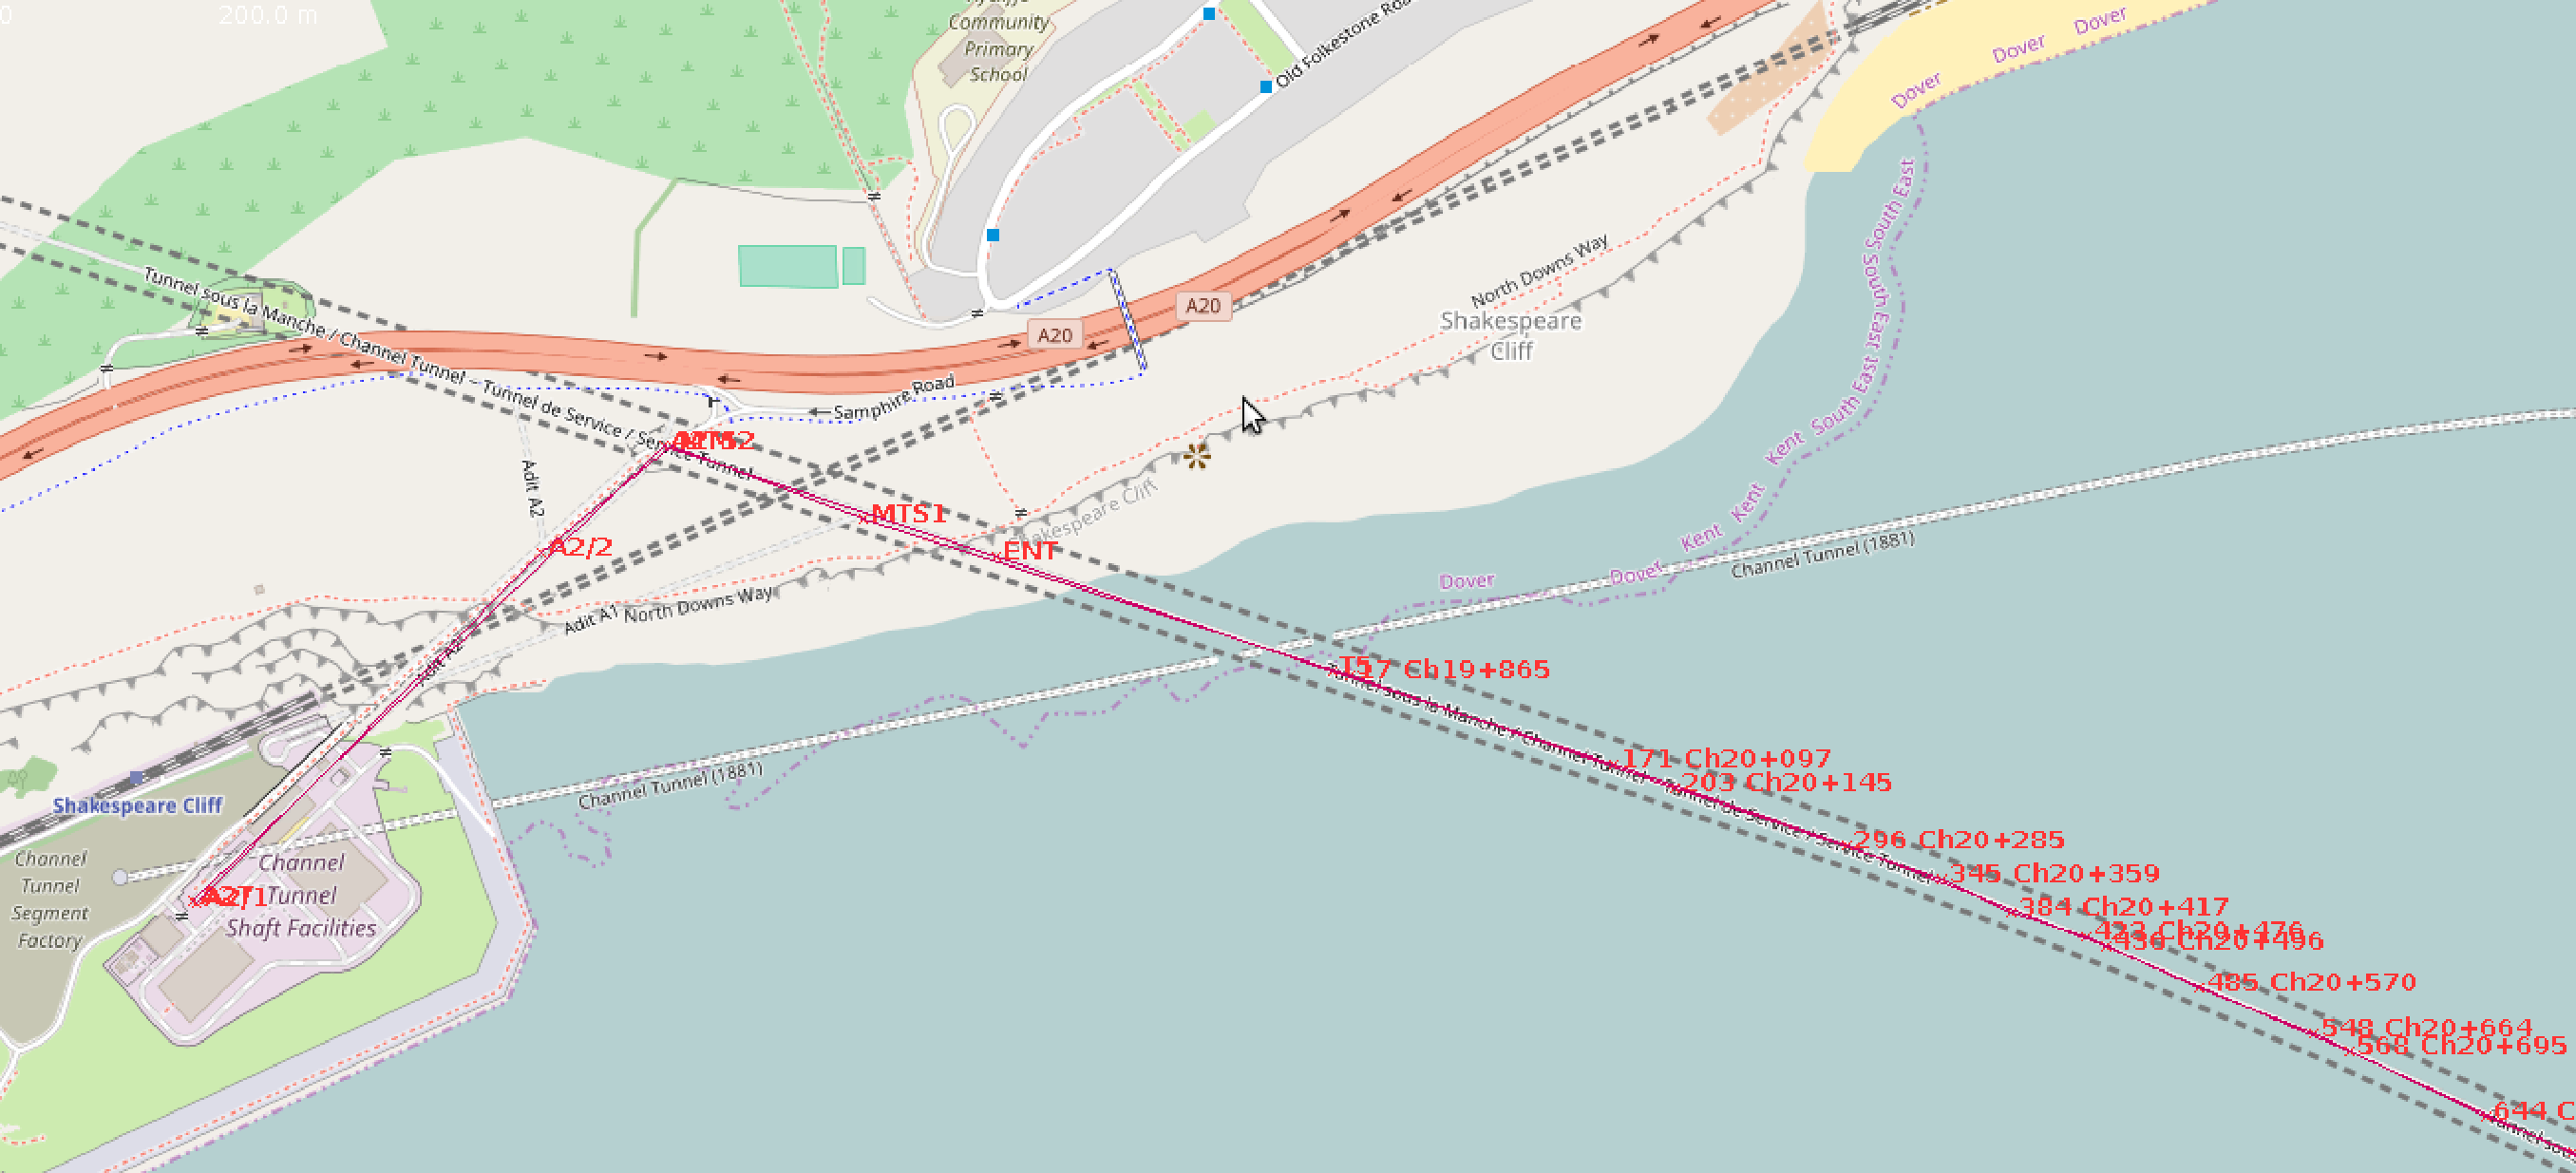
\includegraphics[width=15.1cm]{shakespeare-cliff-cropped}
  \vspace{-0.5em}
  \caption{Channel Tunnel: Shakespeare Cliff, tunnels close to Dover on the British coast (OpenStreetMap, \textsc{cc-by-sa}). 1989/1990 survey traverses in red.}
  \label{fig:osm-chunnel-traverse}
\end{figure*}

%\IEEEtriggeratref{6}

\bibliographystyle{IEEEtran}
\bibliography{sladen-eol2017-tunnels2}


\end{document}


